% !TEX root = template.tex

\section{Introduction}

Here goes the introduction. We also cite the nice book by \citet{Pinedo:2012}.
This might be a book with interesting topics, but concurrent time-stamping has also been addressed before~\cite{Dolev97}.
In this work, \citet{Dolev97} presented the first bounded implementation of a concurrent time-stamp system.

\section{Scheduling Algorithm}

\subsection{Formal Definitions}

\citet*{Chen2017} view a data analytic \emph{job} simply as a number of \emph{tasks} that comprise it. These tasks are further separated into consecutive \emph{stages}, where the future stages depend on the results of the past stages. In other words, the tasks from a single stage must wait for the tasks from all the previous stages to complete. On the contrary, within a single stage the tasks are \emph{independent} of each other and therefore could be executed in parallel.

\citet{Chen2017} further describe a geographically distributed datacenter as a group of independent datacenters connected by a network. Each single datacenter from this group consists of a number of available \emph{computing slots}. Furthermore, the network that connects the pairs of datacenters is expected to have significantly \emph{lower bandwidth} than the local network of each individual datacenter. This means that transferring large amounts of data between different datacenters takes a lot of time. Finally, in order to execute a task, it must be provided with a computing slot and the necessary input data. The input data for every task is also hosted by some datacenter(s). If it so happens that a task is assigned to a datacenter that does not hold the entire input data for that task, the missing parts will have to be transferred across the inter-datacenter network.

\subsection{Optimization Problem}
\subsection{Proposed Scheduling Algorithm}

%% Table~\ref{tab:related_algorithms} shows a summary of related algorithms.

%% \begin{table}[h]
%% \centering
%% \captionabove{Related algorithms and their complexity.}
%% \label{tab:related_algorithms}
%% \begin{tabular}{ll}
%% \toprule 
%% algorithm & complexity \\
%% \midrule
%% algorithm Y & $\mathcal{O}(n)$ \\
%% algorithm Z & $\mathcal{O}(n \log{n} )$ \\
%% \bottomrule
%% \end{tabular}
%% \end{table}

\section{Evaluation of the Scheduling Algorithm}


%% \subsection{Evaluating the Running Time of Algorithm X}

%% The run-time of our algorithm is shown in Figure~\ref{fig:runtime}.
%% We can observe that the run-time of our algorithm increases linearly with the message size.
%% Since we target a system with a run-time of less than \SI{10}{\second}, the maximum message size should be \SI{128}{\byte}.

%% \begin{figure}[h]
%% \centering
%% 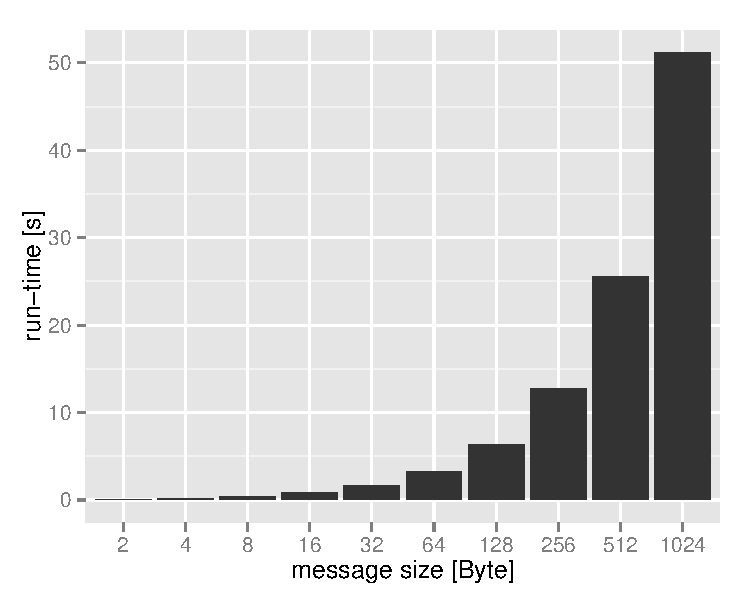
\includegraphics[width=.5\linewidth]{figures/runtime}
%% \caption{Run-time of algorithm X on machine Y.}
%% \label{fig:runtime}
%% \end{figure}

%% \subsection{Evaluating the Space Requirements of Algorithm X}

%% Now, we investigate the space requirements of the algorithms listed in Table~\ref{tab:related_algorithms}.


\section{Summary}
We summary the contribution of the papers and this seminar paper.
